\begin{figure}[t]
  \centering
  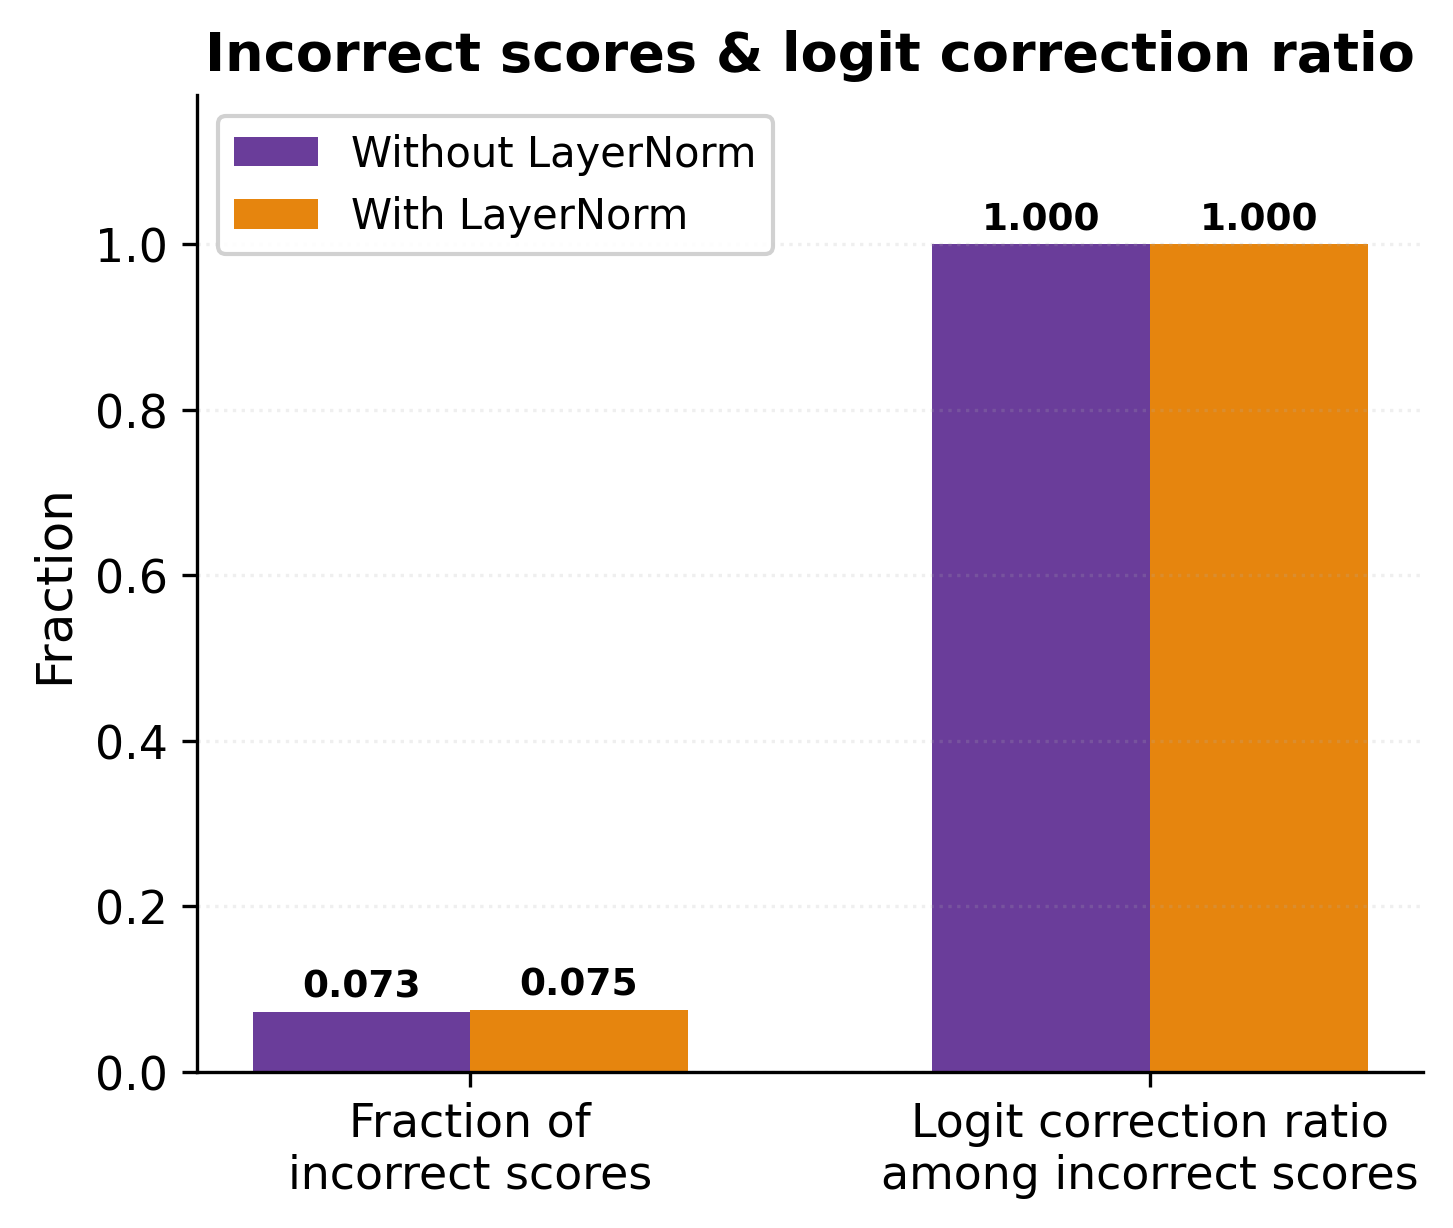
\includegraphics[width=0.48\textwidth]{results/cinclogits/compare_cinclogits.png}
  \caption{Comparison of incorrect attention scores and logit correction between models trained with and without layer normalization. \textbf{(Left)}~Fraction of output positions where the attention mechanism assigns the highest score to an incorrect previous token. \textbf{(Right)}~Among those incorrect-score positions, the fraction where the model's final logit still produces the correct prediction (logit correction ratio). The model with layer normalization achieves a perfect correction ratio of~$1.0$, indicating that its MLP layers fully compensate for attention errors, whereas the model without layer normalization occasionally fails to correct them.}
  \label{fig:cinclogits}
\end{figure}
